\documentclass{fkssolpub}

\usepackage[czech]{babel}
\usepackage{fontspec}
\usepackage{fkssugar}
\usepackage{amsmath}
\usepackage{graphicx}

\renewcommand{\d}{\, \mathrm{d}}
\renewcommand{\angle}{\sphericalangle}

\author{Ondřej Sedláček}
\school{Gymnázium Oty Pavla} 
\series{3}
\problem{C} 

\begin{document}

Jako první si musíme uvědomit, jaká je množina bodů, ve které mohou mít náhodně vykrojené perníčky střed. Víme, že středy musí být od každé strany vzdáleny alespoň $0{,}25$ m, a tedy množina možných středů je čtverec o straně délky $0{,}5$ m. Následně víme, že pokud budeme moci vykrojit oba perníčky, pak vzdálenosti jejich středů bude alespoň $0{,}5$ m. Tedy abychom zjistili pravděpodobnost, že umíme vykrojit další perníček, musíme zjistit poměr velikosti množiny středů, kdy existuje ještě nějaký střed, který je půl metru vzdálený, s velikosti množiny všech středů.

Je zřejmé, že pokud máme nějaký bod ve čtverci, pak nejvzdálenější bod, který leží v daném čtverci, je vždy jeden z jeho vrcholů. Tedy pokud alespoň jeden vrchol leží ve vzdálenosti větší než půl metru, můžeme vyříznout další perníček. Tím pádem množina středů, kdy nezbyde místo na další perníček, je průnik kruhů se středy ve vrcholech s poloměrem půl metru: 
\begin{figure}[h!]
  \begin{center}
    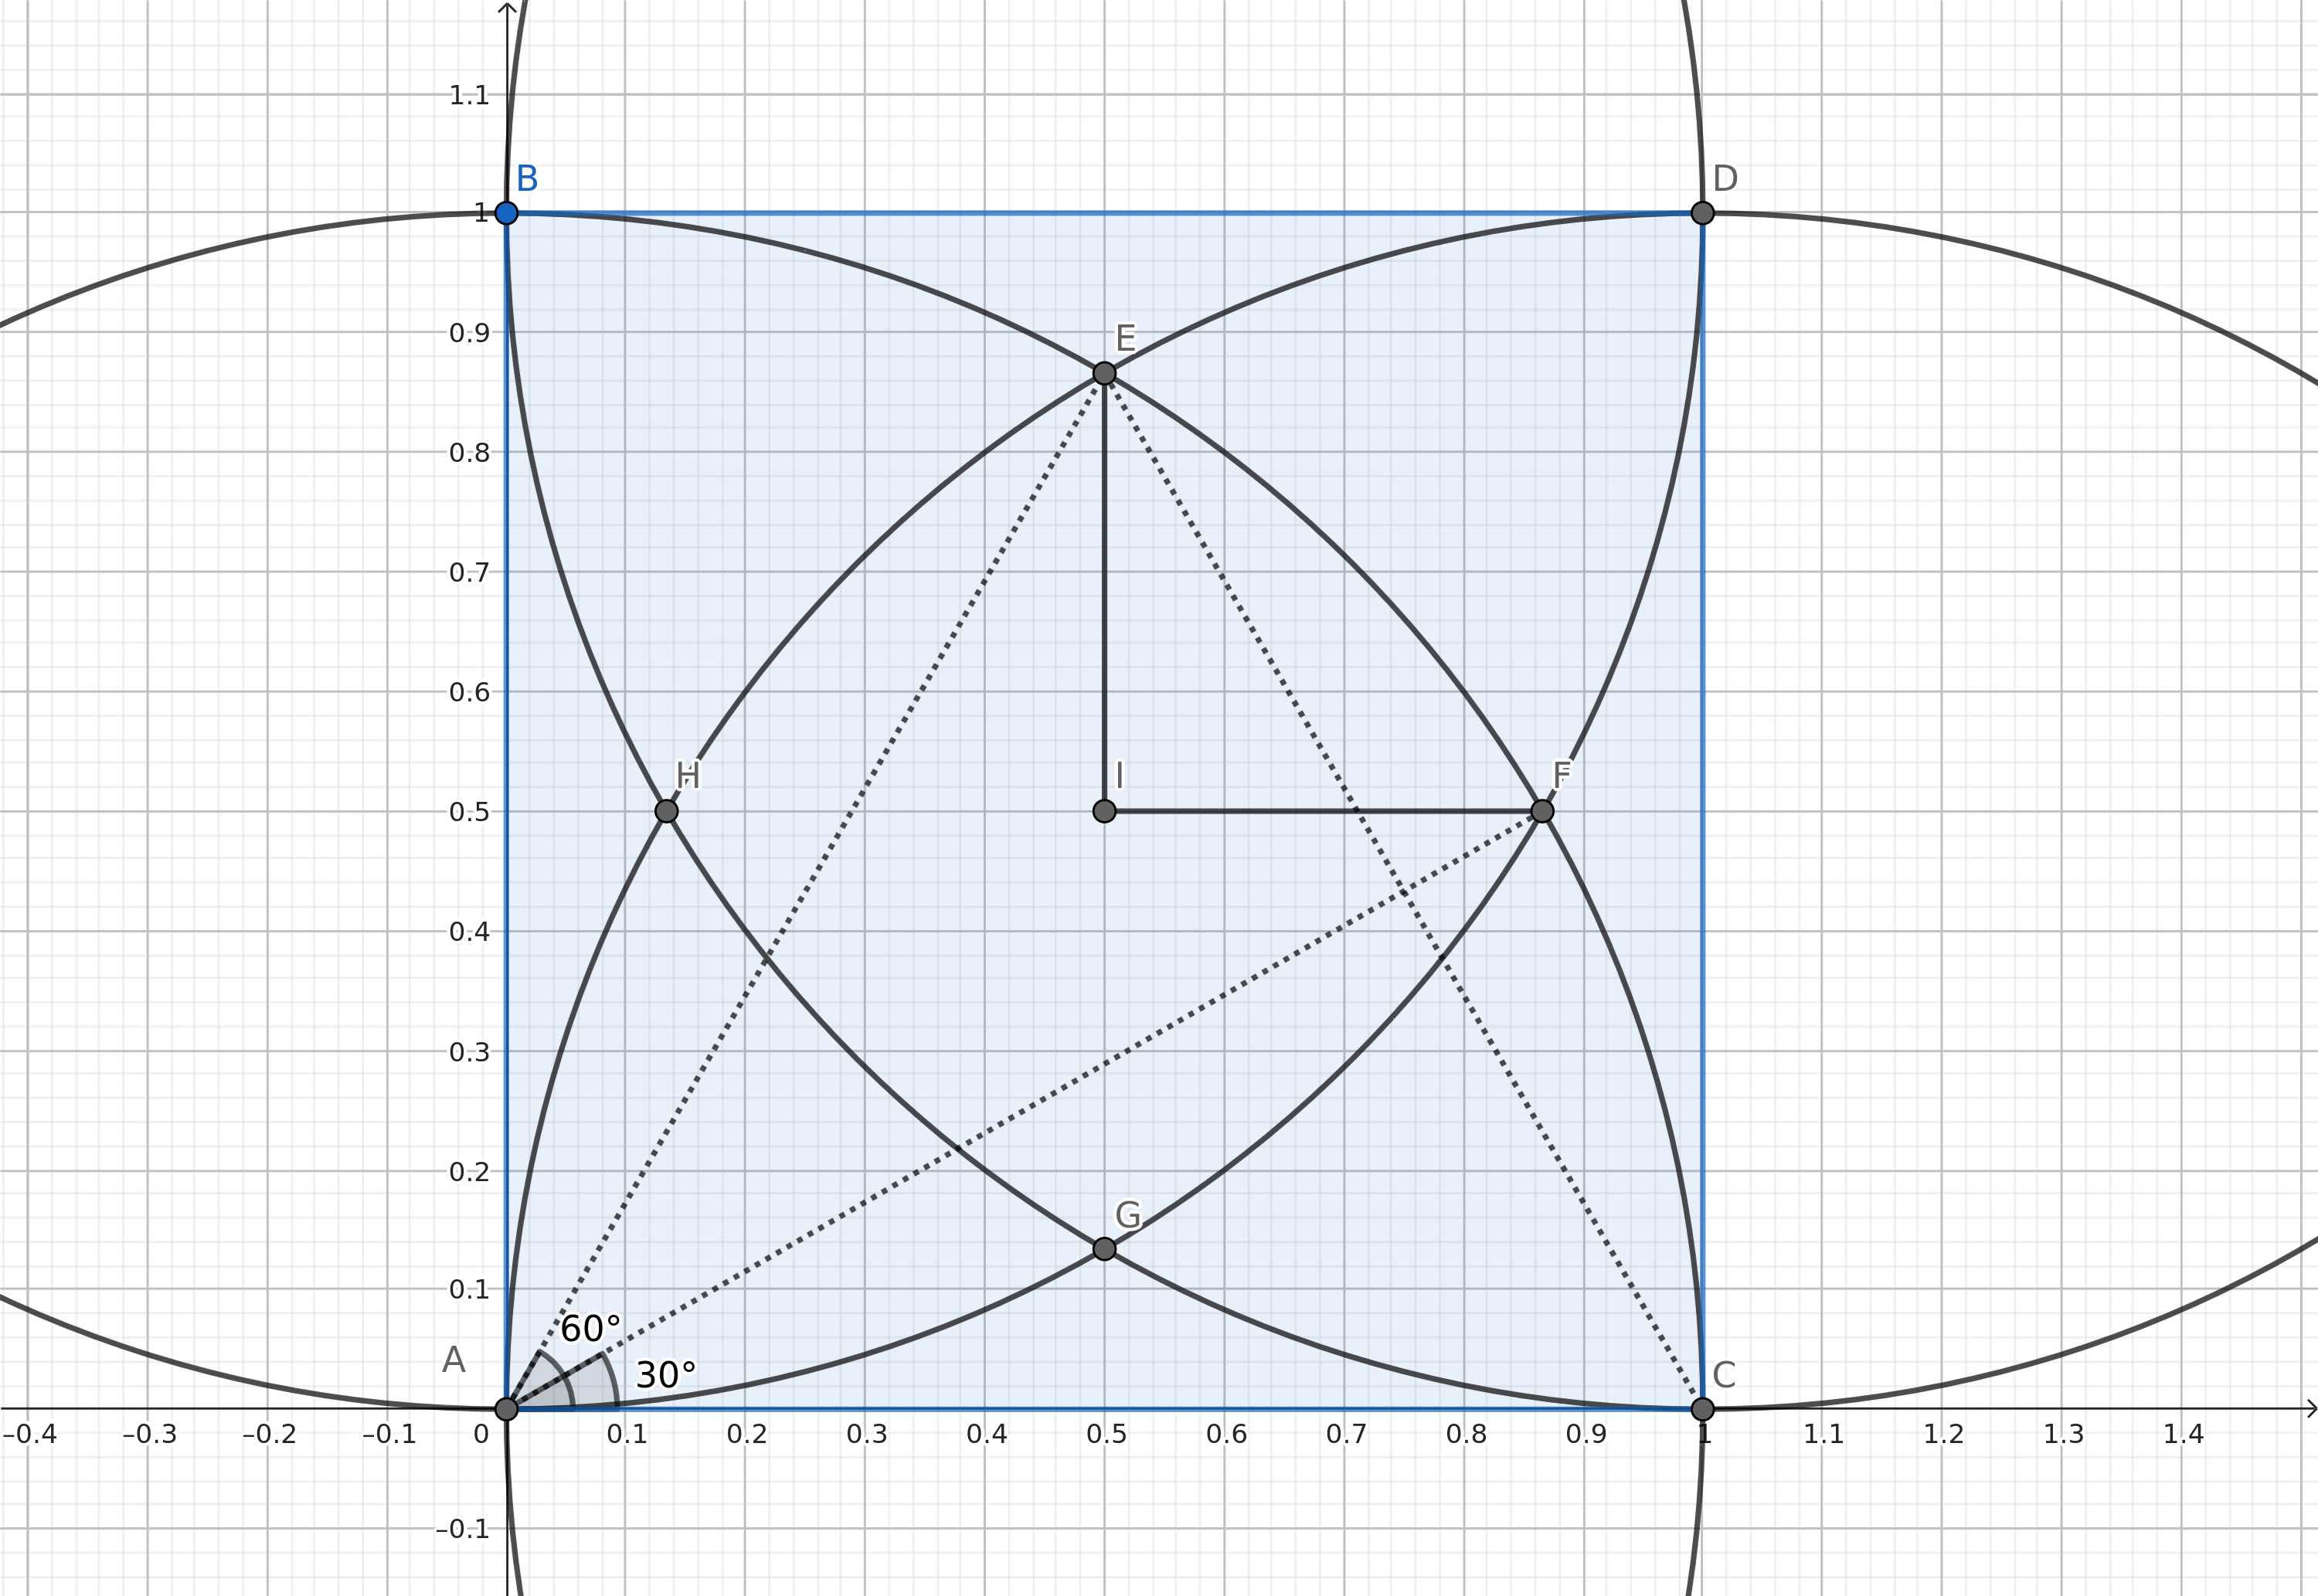
\includegraphics[width=0.95\textwidth]{C-fig.png}
  \end{center}
  \caption{}\label{fig:1}
\end{figure}

Nechť teď pracujeme v takových souřadnicích, kdy délka strany této krychle bude 1. Pak pravděpodobnost, že nebudeme moci vyříznout další perníček, je rovna obsahu průniku všech kružnic. A jelikož je tento útvar symetrický, stačí nám vypočítat jen jeho část $EFI$, tedy:

\[
p' = 4 S_{EFI}
\]

Víme, že $|\angle CAE| = \frac{\pi}{3}$ a $|\angle CAF| = \frac{\pi}{6}$, jelikož $CAE$ a $ABF$ jsou rovnostranný trojúhelníky, proto:

\[
  S_{EFI} = \int_{\cos \frac{\pi}{3}}^{\cos \frac{\pi}{6}} \sqrt{1 - x^2} - \frac{1}{2} \; \d x
\]

Po substituci $x = \cos \theta$ a $\d x = - \sin \theta \d \theta$ dostaneme:

\[
  S_{EFI} = - \int_{\frac{\pi}{3}}^{\frac{\pi}{6}} \left( \sqrt{1 - \cos^2 \theta} - \frac{1}{2} \right) \; \sin \theta \d \theta = - \int_{\frac{\pi}{3}}^{\frac{\pi}{6}} \sin^2 \theta \d \theta - \left[ \frac{1}{2} \cos \theta \right]_{\frac{\pi}{3}}^{\frac{\pi}{6}}
\]

Integrál, který jsme právě dostali, vyřešíme pomocí metody per partes:

\[
  \int \sin^2 \theta \d \theta = \int 1 \d \theta - \int \cos^2 \theta \d \theta = \theta - \left(- \sin \theta \cos \theta + \int \sin^2 \theta \d \theta \right)
\]
\[
  2 \int \sin^2 \theta \d \theta = \theta - \sin \theta \cos \theta
\]
\[
  \int \sin^2 \theta \d \theta = \frac{1}{2} (\theta - \sin \theta \cos \theta)
\]

A tedy:

\[
  S_{EFI} = - \left[\frac{1}{2} (\theta - \sin \theta \cos \theta)\right]_{\frac{\pi}{3}}^{\frac{\pi}{6}} - \left[ \frac{1}{2} \cos \theta \right]_{\frac{\pi}{3}}^{\frac{\pi}{6}} = \frac{\pi}{12} - \frac{\sqrt{3}}{4} + 1
\]

Tedy pravděpodobnost, že budeme moci vyříznout další perníček, je:

\[
  p = 1 - p' = 1 - 4 S_{EFI} = 1 - \frac{\pi}{3} + \sqrt{3} - 1 = \sqrt{3} - \frac{\pi}{3} \doteq 0{,}685 = 68{,}5 \%
\]


\end{document}
